\subsection{管理员端功能实现}

管理员端用于平台侧异常处理和可信审计，是 FoodShield 系统区别于普通聊天系统的重要组成部分。管理员端不是普通的聊天明文查看后台，而是以订单摘要、消息哈希、Merkle Root、完整性验证结果和审计日志为核心的可信审计后台。

管理员访问后台前需要先完成登录认证。系统会校验管理员用户名和口令，认证通过后在服务端 Session 中记录管理员状态。所有管理员接口均受权限校验保护，未登录请求无法访问管理员功能。管理员登录、登出、查看订单、生成快照、执行验证和条件溯源等操作均会写入审计日志。

\begin{figure}[H]
    \centering
    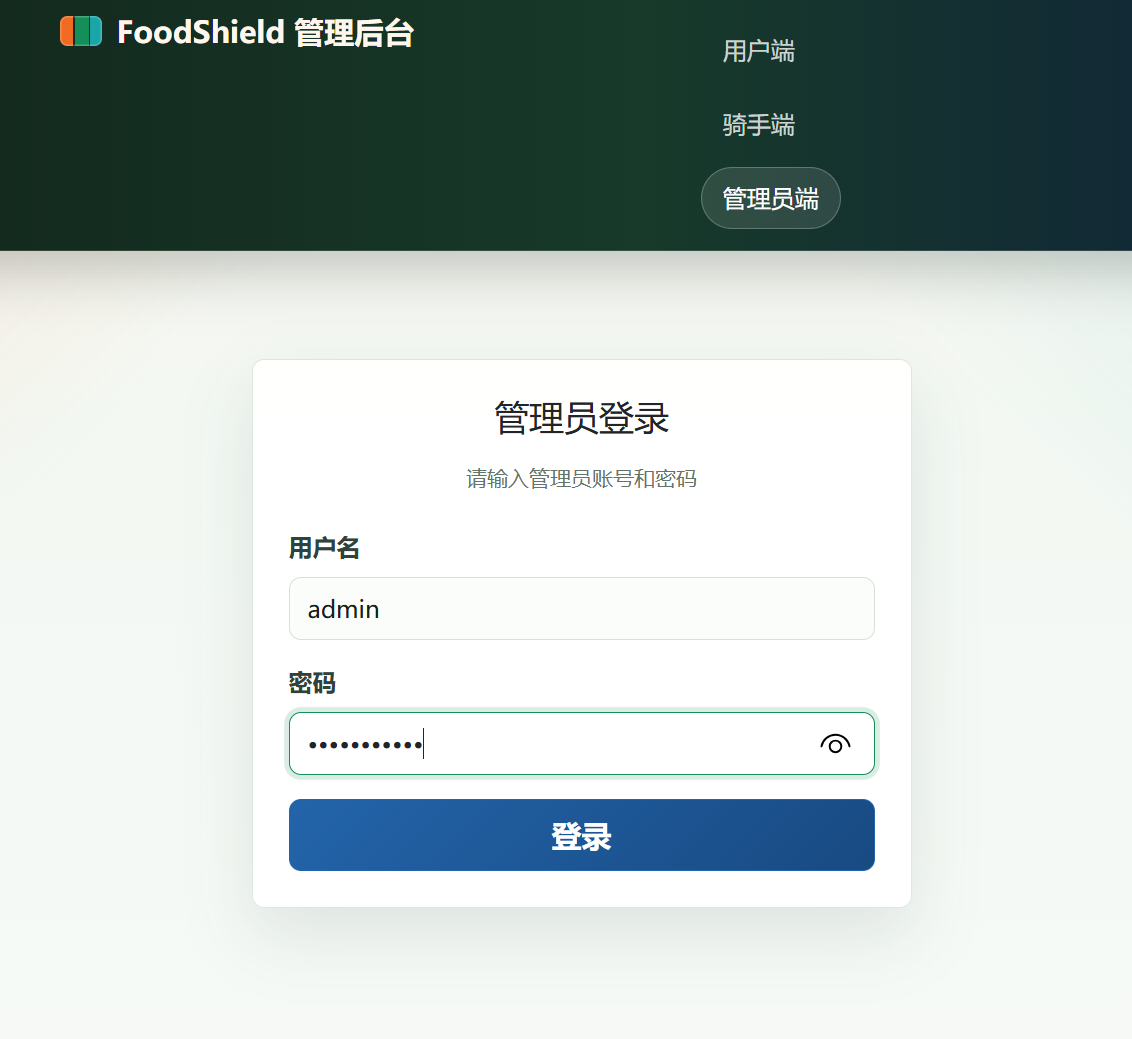
\includegraphics[width=0.8\textwidth]{content/chapter4/admin_login.png}
    \caption{管理员登录界面}
    \label{fig:admin-login}
\end{figure}

登录后，管理员可以根据订单号检索订单摘要和通信日志。管理员默认只能查看消息编号、订单号、发送方角色、时间戳、消息哈希和 Merkle Root 等审计信息，不能通过普通查询接口直接查看通信明文。该设计将审计能力和明文查看能力分离，降低管理员权限带来的二次隐私泄露风险。

\begin{figure}[H]
    \centering
    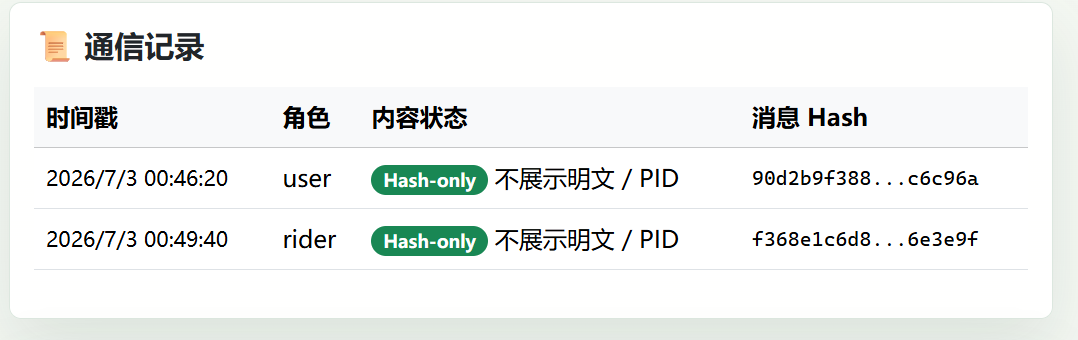
\includegraphics[width=0.95\textwidth]{content/chapter4/admin_message_hash.png}
    \caption{管理员消息摘要查看界面}
    \label{fig:admin-message-hash}
\end{figure}

管理员可以手动为某一订单生成 Merkle Root 快照。系统会读取该订单当前所有消息哈希，按照 Merkle Tree 构建规则计算 Root，并将 Root、订单号、消息数量和快照时间写入 \texttt{audit\_logs} 表。后续完整性验证时，系统会重新计算当前 Root，并与历史快照 Root 进行比对。

\begin{figure}[H]
    \centering
    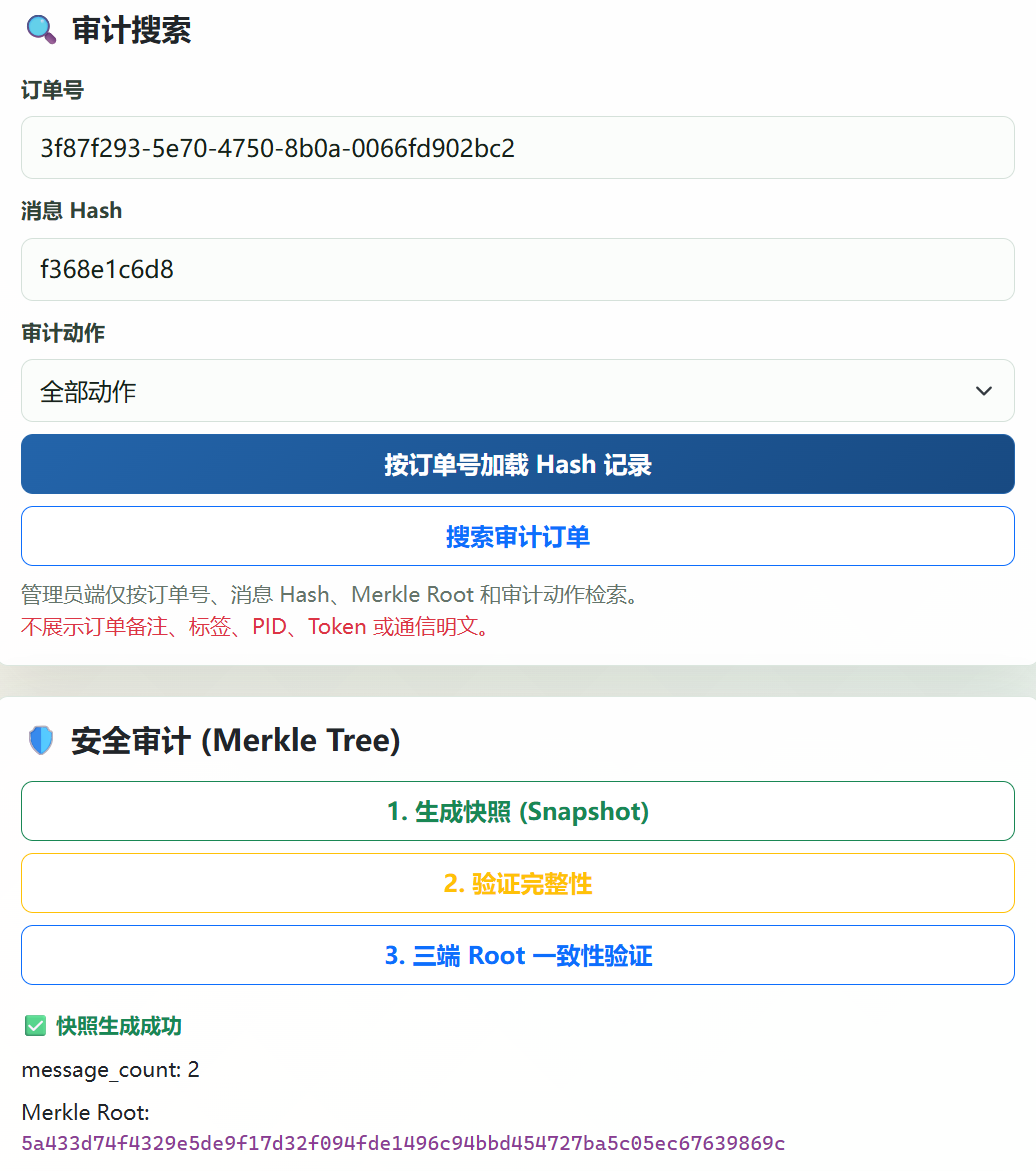
\includegraphics[width=0.95\textwidth]{content/chapter4/admin_merkle_snapshot.png}
    \caption{Merkle Root 快照生成界面}
    \label{fig:admin-merkle-snapshot}
\end{figure}

管理员还可以处理用户端或骑手端提交的溯源申请。管理员执行条件溯源前，系统会先对目标订单执行完整性验证，若验证失败则阻断溯源；若验证通过，再根据投诉关键词检索消息内容，并在关键词命中后完成从订单号到 PID、再从 PID 到真实用户身份的受控映射查询。溯源成功或失败均写入审计日志。

\begin{figure}[H]
    \centering
    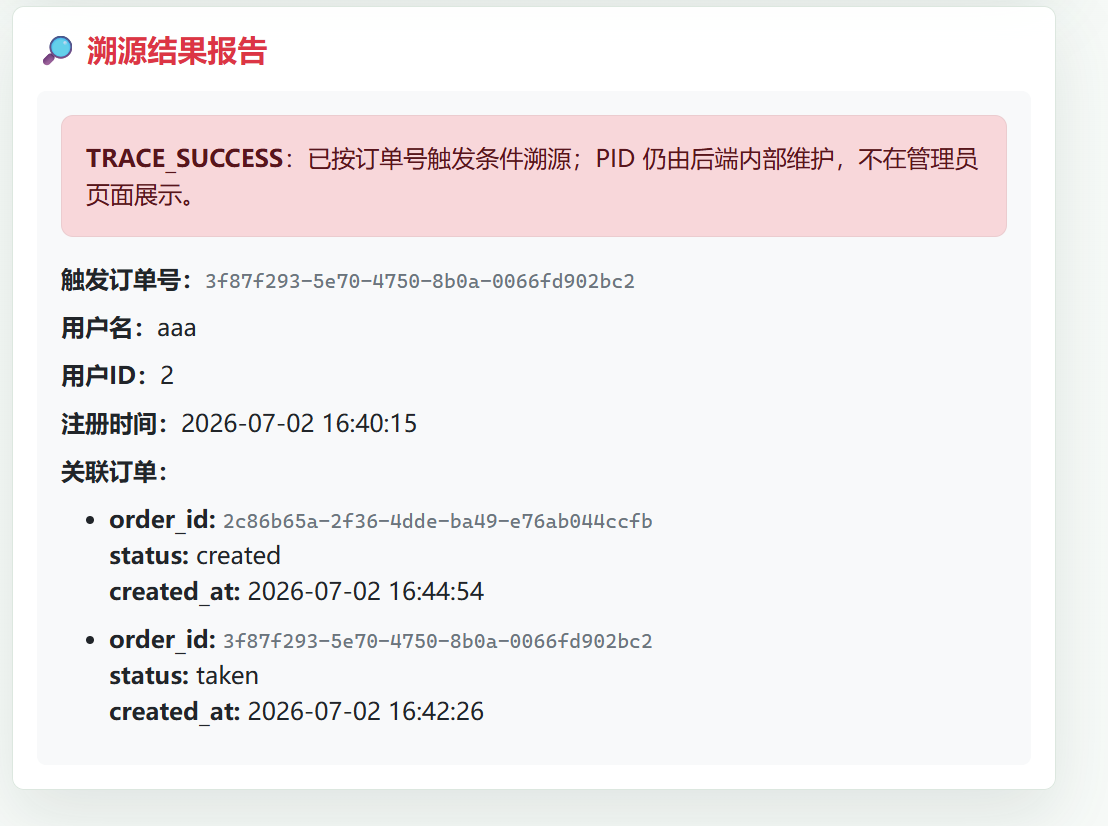
\includegraphics[width=0.95\textwidth]{content/chapter4/admin_trace_result.png}
    \caption{管理员条件溯源界面}
    \label{fig:admin-trace-result}
\end{figure}
